\subsection{Gold Foil Experiments}

Between 1908 and  1913, a number of alpha ($\alpha$) particle scattering experiments were performed by Hans Geiger and Ernest Marsden.
These took the form of shooting $\alpha$  particles at a  incredibly thin piece of gold foil.
Based on the plum pudding model, it was expected that the $\alpha$ particles would not be deflected however this turned out not to be the case at all.
To be fair, most of the $\alpha$ particles did indeed go straight through the gold foil, their trajectory not disturbed in the slightest.
A smaller fraction did get deflected, some by a small angle and others by a large one.
But the astonishing part was that an even smaller fraction, about 1 in 20000, shot right back at the direction the particle gun was shooting from.

\begin{figure}[H]
  % https://en.wikipedia.org/wiki/Rutherford_scattering_experiments#/media/File:Geiger-Marsden_experiment_expectation_and_result.svg
  \centering
  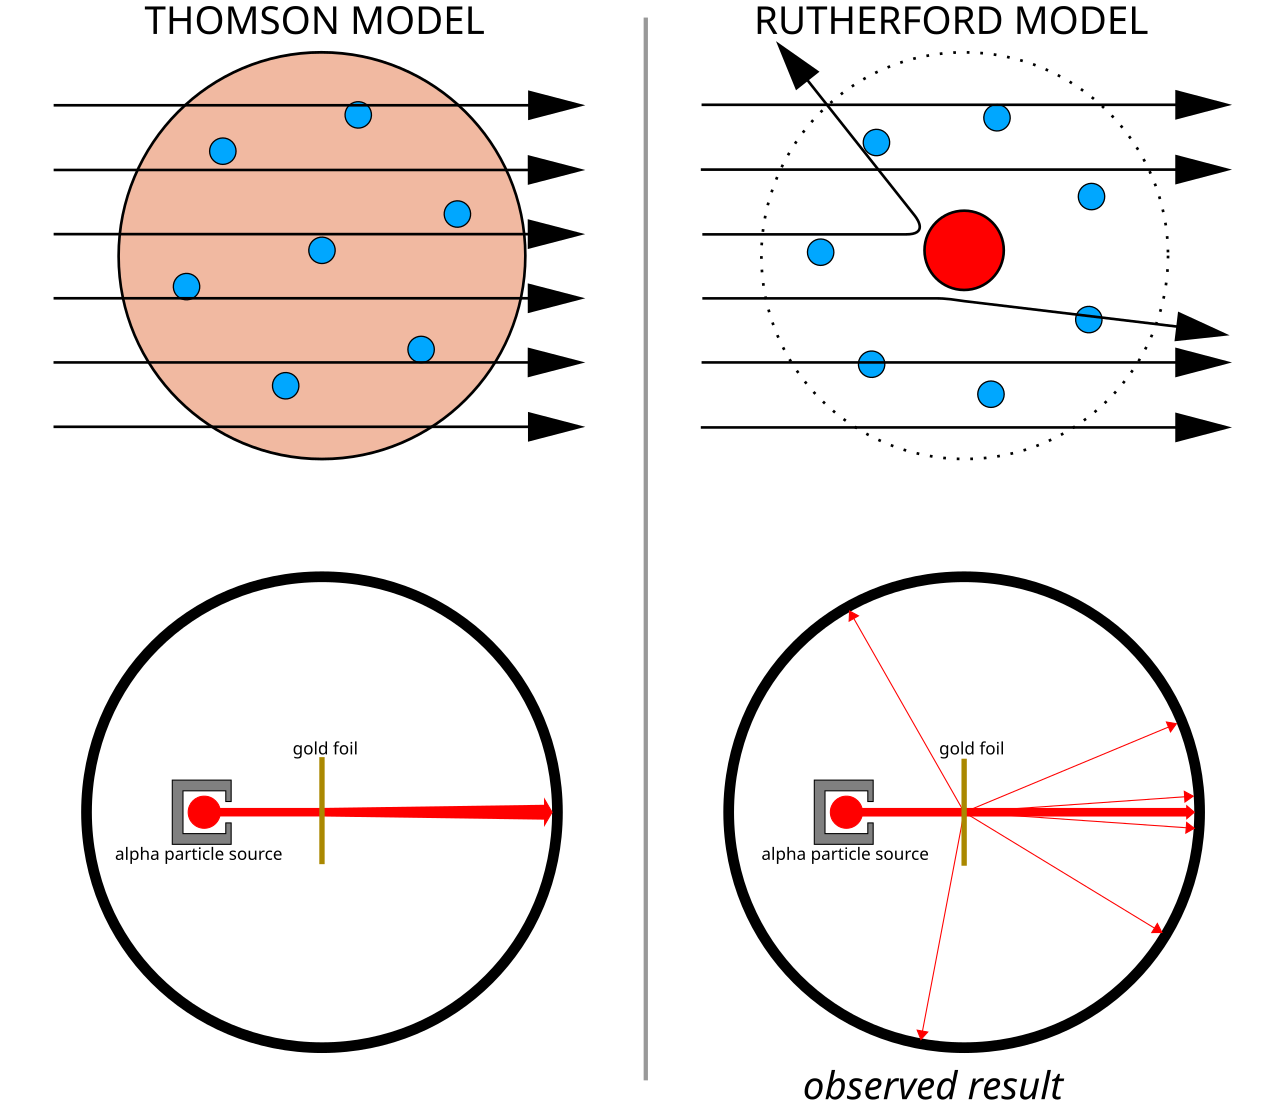
\includegraphics[width=100mm]{figures/goldFoil.png}
  \caption{Cartoon of Gold foil experiment}
  \label{goldFoil}
\end{figure}

